% !TEX root = Informatik-3.tex
\section{Speicher}


\subsection{DRAM}
Dynamisches RAM. 
Wird gelöscht wenn 
\begin{itemize}\itemsep0em
		\item Versorgungsspannung abgeschaltet
		\item Speicherinhalt nicht gerefresht wird
\end{itemize}	

Preiswert, geringer Platzbedarf $\rightarrow$ Arbeitsspeicher.

Zugriffszeiten: 5-20ns (einzelnes Bit).

Besteht aus Kondensator und Transistor.

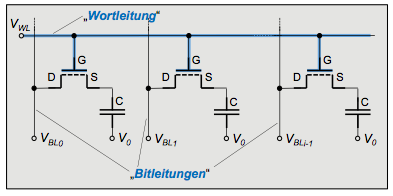
\includegraphics[width=\linewidth]{dram.png}

\subsubsection{DDR(x)-SDRAM}
Datenübertragung bei fallender und steigender Flanke $\rightarrow$ 2 \^ x * schneller

Niedrigere Betriebsspannung

Latenz bei gleichem Takt etwas höher.

\subsection{SRAM}
Speicherinhalt geht verloren wenn die Versorgungsspannung abgeschaltet wird

Kurze Zugriffszeiten, komplex, mehr Strombedarf, wesentlich teurer als DRAM.

$\rightarrow$ Register und Cache.


\subsection{Cache}

\subsubsection{Begriffe}
\begin{description}\itemsep0em
\item [Zeitliche Lokalität] zuletzt benutzte Daten werden wahrscheinlicher bald wieder gebraucht.
\item [Räumliche Lokalität] Sequenzielle Zugriffe häufig
\item[Hit Rate] Trefferrate, Anteil der Speicherzugriffe, die zu einem Treffer im Cache führen.
\item[Miss Rate] Rate der Zugriffe, die zu keinem Treffer im Cache führen. (1- Hit Rate)
\item[Hit Time] Erforderliche Zeit für erfolgreichen Zugriff auf ein Datum im Cache inkl. Test ob vorhanden im Cache.
\item[Miss Penalty] Fehlzugriffsaufwand, erforderliche Zeit für den Austausch eines Blocks im Cache aus nächster Ebene
\end{description}
$\rightarrow$ Miss-Rate reduzieren, Hit Time optimieren (durch Prozessor, Betriebsystem und Compiler)

Wie findet man ein Datum?
\subsubsection{Assoziativer Zugriff (voll)}

Adresse des Datums wird mit allen Adressen der sich im Speicher befindenden Daten parallel verglichen und bei Match Datum unmittelbar gelesen / geschrieben.

$\rightarrow$  braucht zu jedem Datum zusätzlich die Adresse ("Tag") + valid bit.

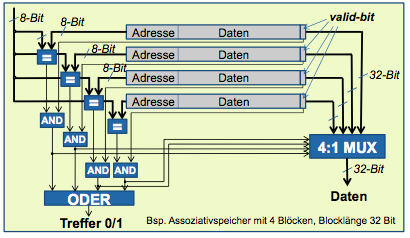
\includegraphics[width=\linewidth]{assozativspeicher.png}

\subsubsection{Direktabbildend}

Jeder Adresse im Speicher wird eine Position im Cache zugeordnet. Z.b. durch modulo realisiert

Tag (Cache-Blocknummer) = (Block-Adresse) \% (Anzahl Blöcke im Cache)

Index (Blockadresse) = (Byteadresse) / (Bytes pro Block) (abgerundet)

Index Anzahl (Blockanzahl) = Cachegrösse / Blockgrösse

Indexlänge = log(Blockanzahl)

Blockgrösse = Blockanzahl * Wortlänge

Länge Wortoffset = log(Worte pro Block)

Länge Byteoffset = log(Wortlänge)

Tag-Grösse  = Adresslänge - Indexlänge - länge Wortoffset + länge byteoffset

Bits = Blockanzahl * (Blockgrösse + Tag-Grösse + Flag-Bits)

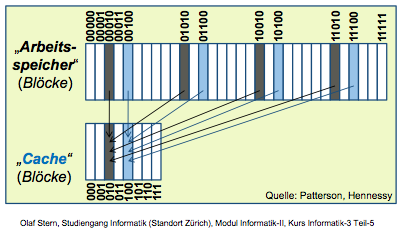
\includegraphics[width=\linewidth]{direktabbildend.png}

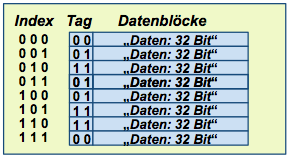
\includegraphics[width=120px]{direktabbildend2.png}
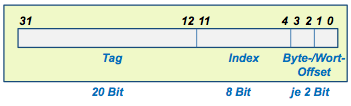
\includegraphics[width=120px]{direktabbildend3.png}

\subsubsection{Satzassoziativ}

Mischform, Block kann auf eine vorgegebene Anzahl von Positionen beliebig abgelegt werden.

Suche:
\begin{itemize}\itemsep0em
		\item Block wird direkt auf Satz abgebildet
		\item Innerhalb der Positionen des Satzes wird assoziativ gesucht.
\end{itemize}	
Typische Satzgrösse: 2 oder 4 Positionen.

1-fach satzassoziativ $\rightarrow$  Direktzugriff

n-fach satzassoziativ mit n Blöcken $\rightarrow$  voll-assozativ

\subsubsection{Verdrängung bei assoziativ und satzassoziativ}
\begin{itemize}\itemsep0em
\item Least recently used (LRU)
\item Least frequently used (LFU)
\item First in first out (FIFO) $\rightarrow$  häufig genutzt, weil einfach.
\end{itemize}	

Bits = Satzanzahl * (Satzgrösse + Tag-Grösse + Flag-Bits)

Flag-Bits: Valid-Bit, FIFO-Bit



\subsubsection{Lesezugriffe - Optimierungen}
\begin{description}\itemsep0em
\item[Early-Restart] Nach Fehlzugriff Programmausführung fortgesetzt, wenn angefordertes Wort des Blockes geladen wird. Folgende Wörter werden just in time geladen. $\rightarrow$ Gut für Zugriffe auf Befehle (sequenziell)
\item[Requested Word First] Bei Fehlzugriff angefordertes Wort zuerst. Anschliessend Rest. (aufwendig)
\end{description}

\subsubsection{Schreibzugriffe}

Komplexer, Gefahr der Inkonsistenz von Cache und Speicher.

\begin{description}\itemsep0em
\item[Write-through] Schreibvorgang immer auch auf den Speicher $\rightarrow$ schlechte Performance.
\item[Write Puffer] Bei Schreiben Daten in Cache und Schreibpuffer, Programm wird dann fortgesetzt. 
\item[Write Back] nur in den Cache schreiben, Programm fortsetzen und Block mit dirty bit markieren. Wird gespeichert, wenn Block überschrieben.
\item[DMA] Direct Memory Access, Peripheriegeräte kann direkt auf Daten im Speicher ohne CPU zugreifen.
\end{description}

\subsubsection{Mehrstufige Caches}

kleiner, schneller Cache beim Prozessor $\rightarrow$ Optimierung der Hit Time

grösserer, langsamerer zweiter Cache auf dem Mainboard $\rightarrow$  Optimierung des Fehlzugriffaufwandes

\subsubsection{Cache-Leistung}

t\_ohneC = (1-A\_S) * T\_C +A\_S * T\_S

t\_mitC =(1-A\_S)* T\_C +A\_S * (R\_hit * t\_hit +(1-R\_hit)* t\_miss)

\begin{description}\itemsep0em
\item[A\_S] Zugriffe auf Speicher
\item[T\_C] Zugriffszeit auf Cache
\item[T\_S] Zugriffszeit auf Speicher
\end{description}

mit zwei caches:

t = (1 - A\_S) * T\_C + A\_S * (R\_hit\_C\_1 * t\_hit\_C\_1 + (1 - R\_hit\_C1) * (R\_hit\_C2 * t\_hit\_C2 + (1 - R\_hit\_C2) * t\_miss\_C2))






